\documentclass{beamer}\usepackage[]{graphicx}\usepackage[]{color}
%% maxwidth is the original width if it is less than linewidth
%% otherwise use linewidth (to make sure the graphics do not exceed the margin)
\makeatletter
\def\maxwidth{ %
  \ifdim\Gin@nat@width>\linewidth
    \linewidth
  \else
    \Gin@nat@width
  \fi
}
\makeatother

\definecolor{fgcolor}{rgb}{1, 0.894, 0.769}
\newcommand{\hlnum}[1]{\textcolor[rgb]{0.824,0.412,0.118}{#1}}%
\newcommand{\hlstr}[1]{\textcolor[rgb]{1,0.894,0.71}{#1}}%
\newcommand{\hlcom}[1]{\textcolor[rgb]{0.824,0.706,0.549}{#1}}%
\newcommand{\hlopt}[1]{\textcolor[rgb]{1,0.894,0.769}{#1}}%
\newcommand{\hlstd}[1]{\textcolor[rgb]{1,0.894,0.769}{#1}}%
\newcommand{\hlkwa}[1]{\textcolor[rgb]{0.941,0.902,0.549}{#1}}%
\newcommand{\hlkwb}[1]{\textcolor[rgb]{0.804,0.776,0.451}{#1}}%
\newcommand{\hlkwc}[1]{\textcolor[rgb]{0.78,0.941,0.545}{#1}}%
\newcommand{\hlkwd}[1]{\textcolor[rgb]{1,0.78,0.769}{#1}}%
\let\hlipl\hlkwb

\usepackage{framed}
\makeatletter
\newenvironment{kframe}{%
 \def\at@end@of@kframe{}%
 \ifinner\ifhmode%
  \def\at@end@of@kframe{\end{minipage}}%
  \begin{minipage}{\columnwidth}%
 \fi\fi%
 \def\FrameCommand##1{\hskip\@totalleftmargin \hskip-\fboxsep
 \colorbox{shadecolor}{##1}\hskip-\fboxsep
     % There is no \\@totalrightmargin, so:
     \hskip-\linewidth \hskip-\@totalleftmargin \hskip\columnwidth}%
 \MakeFramed {\advance\hsize-\width
   \@totalleftmargin\z@ \linewidth\hsize
   \@setminipage}}%
 {\par\unskip\endMakeFramed%
 \at@end@of@kframe}
\makeatother

\definecolor{shadecolor}{rgb}{.97, .97, .97}
\definecolor{messagecolor}{rgb}{0, 0, 0}
\definecolor{warningcolor}{rgb}{1, 0, 1}
\definecolor{errorcolor}{rgb}{1, 0, 0}
\newenvironment{knitrout}{}{} % an empty environment to be redefined in TeX

\usepackage{alltt}
\usepackage{../371g-slides}
\title{Logistic Regression 2}
\subtitle{Lecture 16}
\author{STA 371G}
\IfFileExists{upquote.sty}{\usepackage{upquote}}{}
\begin{document}
  
  

  \frame{\maketitle}

  % Show outline at beginning of each section
  \AtBeginSection[]{ 
    \begin{frame}<beamer>
      \tableofcontents[currentsection]
    \end{frame}
  }

  %%%%%%% Slides start here %%%%%%%

  \begin{darkframes}
    \begin{frame}{Should pot be legal?}
      \begin{columns}[onlytextwidth]
        \column{.5\textwidth}
          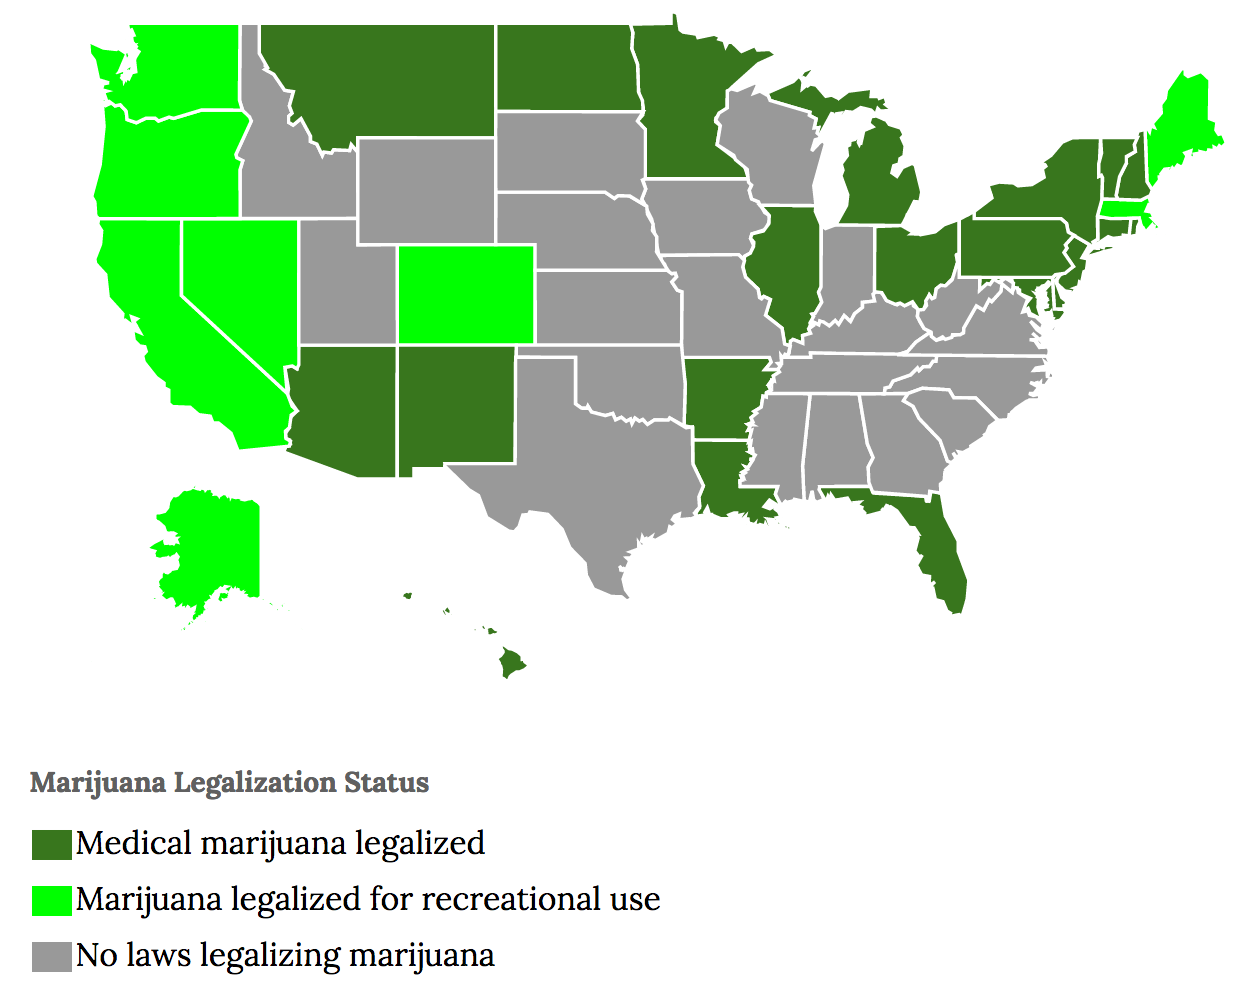
\includegraphics[width=2in]{map}

          \begin{center}
            \fontsize{8}{8} 
            \href{http://www.governing.com/gov-data/state-marijuana-laws-map-medical-recreational.html}{(Map source)}
          \end{center}
        
        \column{.5\textwidth}
          \begin{itemize}
            \item The General Social Survey is an annual survey of attitudes and behaviors that has been conducted since the 1970s
            \item Let's use the GSS to examine the question of whether Americans think pot should be legalized
            \item An increasing number of states have done so already!
          \end{itemize}
      \end{columns}
    \end{frame}

    \begin{frame}
      Response variable:
      \begin{itemize}
        \item \textbf{legal}: Answer to ``Do you think the use of marijuana should be made legal or not?'' \pause\alert{This is binary (yes/no), so we'll need to use logistic regression.}
      \end{itemize}

      \pause
      Predictor variables:
      \begin{itemize}
        \item \textbf{year}: The year of the survey (1975-2014)
        \item \textbf{age}: The age of the respondent
        \item \textbf{schooling}: Number of years of schooling (e.g., 12 = HS degree, 16 = bachelor's)
        \item \textbf{philosophy}: Political philosophy (on the spectrum of liberal to conservative)
      \end{itemize}
      \note{LC questions 2-4}
    \end{frame}

    \begin{frame}[fragile]
      Let's start by building a model using only the \texttt{year} variable:
      \fontsize{8}{8}\selectfont
\begin{knitrout}
\definecolor{shadecolor}{rgb}{0.137, 0.137, 0.137}\begin{kframe}
\begin{alltt}
\hlstd{model1} \hlkwb{<-} \hlkwd{glm}\hlstd{(legal} \hlopt{~} \hlstd{year,} \hlkwc{data}\hlstd{=pot,} \hlkwc{family}\hlstd{=binomial)}
\hlkwd{summary}\hlstd{(model1)}
\end{alltt}
\begin{verbatim}

Call:
glm(formula = legal ~ year, family = binomial, data = pot)

Deviance Residuals: 
    Min       1Q   Median       3Q      Max  
-1.1202  -0.8596  -0.7330   1.3005   1.8827  

Coefficients:
              Estimate Std. Error z value Pr(>|z|)    
(Intercept) -75.022369   2.368408  -31.68   <2e-16 ***
year          0.037183   0.001187   31.34   <2e-16 ***
---
Signif. codes:  0 '***' 0.001 '**' 0.01 '*' 0.05 '.' 0.1 ' ' 1

(Dispersion parameter for binomial family taken to be 1)

    Null deviance: 34665  on 28335  degrees of freedom
Residual deviance: 33646  on 28334  degrees of freedom
AIC: 33650

Number of Fisher Scoring iterations: 4
\end{verbatim}
\end{kframe}
\end{knitrout}
      \note{LC questions 5 and 6}
    \end{frame}

    \begin{frame}[fragile]{Evaluating model fit: Take 1}
      Our baseline prediction percentage is 69.9\% (this is how many cases we'd predict correctly if we just predicted $\text{legal} = 0$ for everyone).

      \bigskip\pause

      How well do we do by using the model?

      \fontsize{9}{9}\selectfont
\begin{knitrout}
\definecolor{shadecolor}{rgb}{0.137, 0.137, 0.137}\begin{kframe}
\begin{alltt}
\hlstd{predicted.legal} \hlkwb{<-} \hlstd{(}\hlkwd{predict}\hlstd{(model1,} \hlkwc{type}\hlstd{=}\hlstr{'response'}\hlstd{)} \hlopt{>=} \hlnum{0.5}\hlstd{)}
\hlstd{actual.legal} \hlkwb{<-} \hlstd{(pot}\hlopt{$}\hlstd{legal} \hlopt{==} \hlnum{1}\hlstd{)}
\hlkwd{sum}\hlstd{(predicted.legal} \hlopt{==} \hlstd{actual.legal)} \hlopt{/} \hlkwd{nrow}\hlstd{(pot)}
\end{alltt}
\begin{verbatim}
[1] 0.6990401
\end{verbatim}
\end{kframe}
\end{knitrout}

      \pause\fontsize{11}{11}\selectfont
      No better than a naive model that just predicts the same for everyone!
    \end{frame}

    \begin{frame}{Evaluating model fit: Take 2}
      Let's also try computing McFadden's pseudo-$R^2$:
      
      \[
        \text{Pseudo-}R^2 = 1 - \frac{\text{residual deviance}}{\text{null deviance}} = 
        1 - \frac{33645.96}{34664.87} = 0.03
      \]

      \bigskip\pause
      Both metrics show us that year does not help us predict attitude towards legalization very well (but we wouldn't expect it to --- why not?)
    \end{frame}

    \begin{frame}{Improving the model}
      Let's add more predictors to the model:
      \begin{itemize}
        \item Years of schooling
        \item Age of respondent
        \item Political philosophy
        \item Gender
      \end{itemize}
      \lc
    \end{frame}

    \begin{frame}[fragile]{Interpreting the coefficients}
      Let's interpret the coefficients:
      \fontsize{9}{9}\selectfont
\begin{knitrout}
\definecolor{shadecolor}{rgb}{0.137, 0.137, 0.137}\begin{kframe}
\begin{alltt}
\hlstd{model2} \hlkwb{<-} \hlkwd{glm}\hlstd{(legal} \hlopt{~} \hlstd{year} \hlopt{+} \hlstd{age} \hlopt{+} \hlstd{schooling} \hlopt{+} \hlstd{philosophy}
                      \hlopt{+} \hlstd{gender,} \hlkwc{data}\hlstd{=pot,} \hlkwc{family}\hlstd{=binomial)}
\end{alltt}
\end{kframe}
\end{knitrout}
\begin{knitrout}
\definecolor{shadecolor}{rgb}{0.137, 0.137, 0.137}\begin{kframe}
\begin{verbatim}
                               Estimate Std. Error z value Pr(>|z|)
(Intercept)                      -80.24       2.56  -31.34     0.00
year                               0.04       0.00   30.66     0.00
age                               -0.02       0.00  -20.96     0.00
schooling                          0.06       0.00   12.52     0.00
philosophyExtremely liberal        1.73       0.08   20.41     0.00
philosophyExtrmly conservative    -0.01       0.10   -0.09     0.93
philosophyLiberal                  1.41       0.06   25.64     0.00
philosophyModerate                 0.60       0.05   13.05     0.00
philosophySlghtly conservative     0.37       0.05    6.95     0.00
philosophySlightly liberal         0.97       0.05   17.99     0.00
genderMale                        -0.02       0.03   -0.55     0.58
\end{verbatim}
\end{kframe}
\end{knitrout}
    \end{frame}

    \begin{frame}[fragile]{Interpreting the coefficients}
      \fontsize{9}{9}\selectfont
\begin{knitrout}
\definecolor{shadecolor}{rgb}{0.137, 0.137, 0.137}\begin{kframe}
\begin{verbatim}
                               Estimate Std. Error z value Pr(>|z|)
(Intercept)                      -80.24       2.56  -31.34     0.00
year                               0.04       0.00   30.66     0.00
age                               -0.02       0.00  -20.96     0.00
schooling                          0.06       0.00   12.52     0.00
philosophyExtremely liberal        1.73       0.08   20.41     0.00
philosophyExtrmly conservative    -0.01       0.10   -0.09     0.93
philosophyLiberal                  1.41       0.06   25.64     0.00
philosophyModerate                 0.60       0.05   13.05     0.00
philosophySlghtly conservative     0.37       0.05    6.95     0.00
philosophySlightly liberal         0.97       0.05   17.99     0.00
genderMale                        -0.02       0.03   -0.55     0.58
\end{verbatim}
\end{kframe}
\end{knitrout}
      \fontsize{11}{11}\selectfont
      All else being equal, being a year older decreases the predicted \emph{odds} that you will support marijuana legalization by 1.8\% (since $e^{-0.018} = 0.982$ and $1-0.982 = 0.018$).
    \end{frame}
    \note{LC questions 8-10}

    \begin{frame}[fragile]{Evaluating model fit: Take 1}
      Recall that our baseline prediction percentage is 69.9\% (this is how many cases we'd predict correctly if we just predicted $\text{legal} = 0$ for everyone).

      \bigskip\pause

      How well do we do by using the model?

      \fontsize{9}{9}\selectfont
\begin{knitrout}
\definecolor{shadecolor}{rgb}{0.137, 0.137, 0.137}\begin{kframe}
\begin{alltt}
\hlstd{predicted.legal} \hlkwb{<-} \hlstd{(}\hlkwd{predict}\hlstd{(model2,} \hlkwc{type}\hlstd{=}\hlstr{'response'}\hlstd{)} \hlopt{>=} \hlnum{0.5}\hlstd{)}
\hlstd{actual.legal} \hlkwb{<-} \hlstd{(pot}\hlopt{$}\hlstd{legal} \hlopt{==} \hlnum{1}\hlstd{)}
\hlkwd{sum}\hlstd{(predicted.legal} \hlopt{==} \hlstd{actual.legal)} \hlopt{/} \hlkwd{nrow}\hlstd{(pot)}
\end{alltt}
\begin{verbatim}
[1] 0.721
\end{verbatim}
\end{kframe}
\end{knitrout}
    \end{frame}

    \begin{frame}{Evaluating model fit: Take 2}
      
      \[
        \text{Pseudo-}R^2 = 1 - \frac{\text{residual deviance}}{\text{null deviance}} = 
        1 - \frac{31593.96}{34664.87} = 0.09
      \]

      \pause\bigskip

      \fontsize{11}{11}\selectfont
      Is it surprising that our measures of model fit are fairly low?
    \end{frame}

    \begin{frame}[fragile]{Testing the overall null hypothesis}
      Like with linear regression, there is an overall null hypothesis for the model that all coefficients (except the intercept) are 0 in the population.

      \bigskip\pause

      To test this, we can use a \emph{likelihood-ratio test} (the likelihood measures how likely we are to see a particular set of data if a particular model is correct).

      \bigskip\pause

      We first have to define a null model (with no predictors), just like we did for stepwise regression:
\begin{knitrout}
\definecolor{shadecolor}{rgb}{0.137, 0.137, 0.137}\begin{kframe}
\begin{alltt}
\hlstd{null} \hlkwb{<-} \hlkwd{glm}\hlstd{(legal} \hlopt{~} \hlnum{1}\hlstd{,} \hlkwc{data}\hlstd{=pot,} \hlkwc{family}\hlstd{=binomial)}
\end{alltt}
\end{kframe}
\end{knitrout}
    \end{frame}

    \begin{frame}[fragile]{Testing the overall null hypothesis}
      Now we can test our current model against the null model: 
      \fontsize{9}{9}\selectfont
\begin{knitrout}
\definecolor{shadecolor}{rgb}{0.137, 0.137, 0.137}\begin{kframe}
\begin{alltt}
\hlkwd{library}\hlstd{(lmtest)}
\hlkwd{lrtest}\hlstd{(null, model2)}
\end{alltt}
\begin{verbatim}
Likelihood ratio test

Model 1: legal ~ 1
Model 2: legal ~ year + age + schooling + philosophy + gender
  #Df LogLik Df Chisq Pr(>Chisq)    
1   1 -17332                        
2  11 -15797 10  3071     <2e-16 ***
---
Signif. codes:  0 '***' 0.001 '**' 0.01 '*' 0.05 '.' 0.1 ' ' 1
\end{verbatim}
\end{kframe}
\end{knitrout}
      \fontsize{11}{11}\selectfont
      \pause
      Since $p< 2\times 10^{-16}$, we can reject the overall model null hypothesis (not surprising since we had many significant coefficients).
    \end{frame}
  \end{darkframes}
\end{document}
